\begin{figure}[ht]
	\centering
	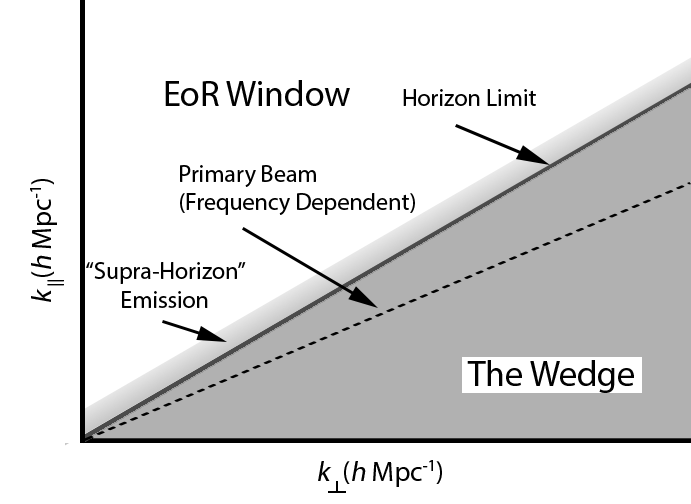
\includegraphics[width=0.9\textwidth]{wedge-diagram.png}
	\caption[Foreground Wedge]{A depiction of the cylindrically averaged 21\,cm power spectrum divided into
					the EoR window and the Wedge. Power from spectrally smooth foregrounds dominate the cosmological
					21\,cm signal at low $k_{\parallel}$ values and bleed into higher $k_{\parallel}$ modes the further
					they are from the field center, extending all the way to the horizon in cases of zenith-pointing
					telescopes such as HERA.}
	\label{fig:wedge}
\end{figure}

\begin{figure}[th]
	\centering
	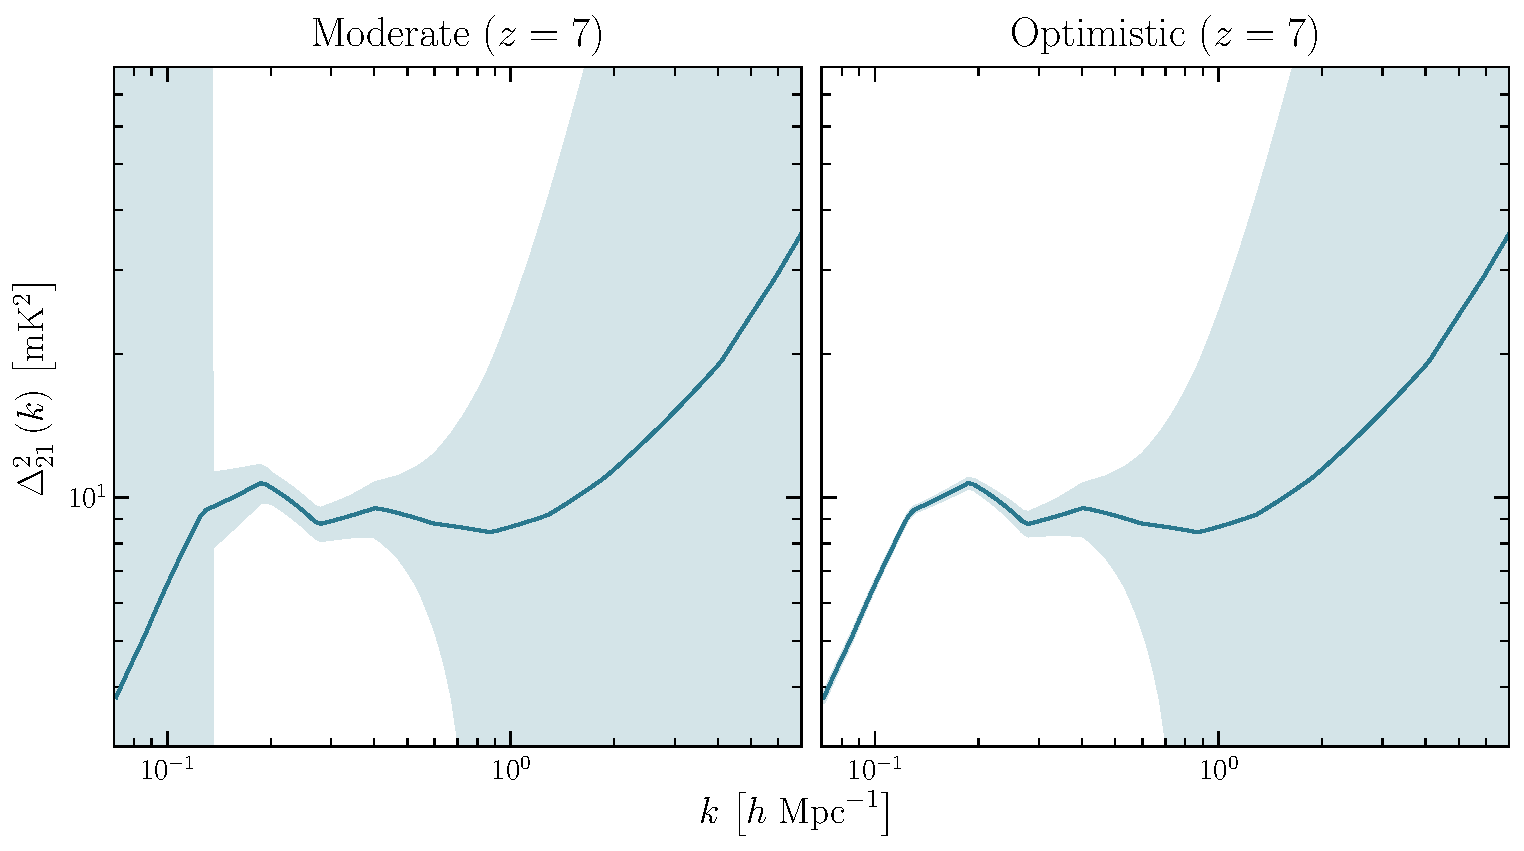
\includegraphics[width=1.0\textwidth]{21cm_errorbars.pdf}
	\caption[Optimistic vs. Moderate Foreground Treatment]{The 21\,cm power spectrum plotted with 1$\sigma$ errors given
																												 observing parameters stated in table BLAH. Here, I compare the
																												 dependence of the two foreground cases on the noise. For the moderate case,
																												 all k-modes within the horizon limit are removed resulting in a complete loss of information on large scales $k \lesssim 0.15 \ h\,\textrm{Mpc}^{-1}$. For the optimistic case, foregrounds extend to the first null in HERA's beam resulting in
																												 a much higher recovery of large scale information.}
	\label{fig:21cm_errors}
\end{figure}

\begin{figure}[th]
	\centering
	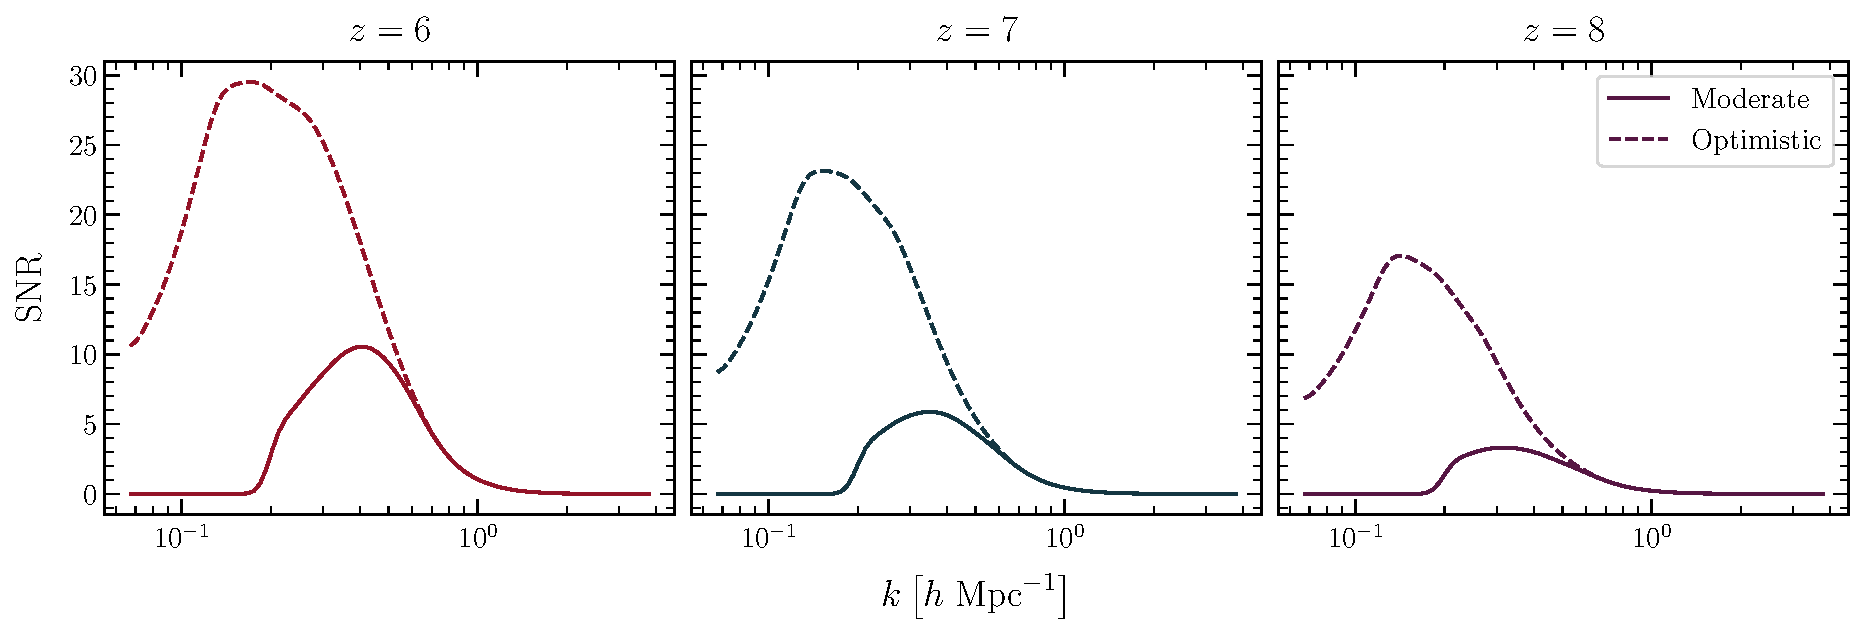
\includegraphics[width=0.95\textwidth]{xcorr_snr.pdf}
	\caption[Cross-Power Spectrum Signal-to-Noise]{Signal to noise estimates for the 21\,cm-\lya\ cross-power spectrum.
	The redshifts $z = [6, 7, 8]$ are plotted for both the optimistic and moderate foreground treatments. These estimates take
	into account the 21\,cm foreground wedge, thermal and sample variance from HERA and SPHEREx, and \lya\ attentuation due to
	absorption in the neutral IGM.}
	\label{fig:snr}
\end{figure}



Here is an explanation of the wedge (\cite{2010ApJ...724..526D}, \cite{2012ApJ...752..137M})

Cross-correlation of reionization-era 21\,cm observations with \lya\ intensity
mapping surveys have the advantage that 21\,cm foregrounds have no correlation with
low redshift interloper lines. Because the two do not correlate, no power from the foregrounds
is added to the cross-power spectrum. However, while the foregrounds don't contribute
to the total cross-power spectrum, they do contribute to the overall variance
of the measurement, and therefore the errors.

\begin{equation}
    k_{\parallel} \approx \theta_{0} k_{\perp} \frac{D_{M} \left( z \right) }{D_H} \frac{E \left( z \right)}{\left(1 + z\right)}
\end{equation}

In the previous section, I calculated the cross-power spectrum for the case where
foreground are completely uncorrelated (don't contribute to the cross-power spectrum
amplitude) and where they did not contribute to the total variance. In this section,
I'll take a more realistic and honest approach to calculating the errors by dealing
with the 21\,cm foregrounds in two different ways. There are two primary methods
that I chose to deal with the foregrounds: by relying on the fact that the foregrounds
are spectrally smooth and thus confined to an area of the 2D power spectrum known
as the wedge and by assuming some imperfect removal method. Each method has advantages
and disadvantages.

In addition to avoiding 21\,cm foregrounds by cutting out k-modes that fall within
the wedge, efforts are being made to model galactic diffuse emission and extragalactic
point sources to directly remove them from the data. This technique is known as
foreground subtraction. While this modeling foregrounds accurately has been shown
to be quite difficult, it gives the added benefit of recovering the foreground
modes that fall within the wedge, increasing the signal to noise of the measurement
at large scales, assuming perfect (or near perfect) foreground subtraction.

While outside the scope of this particular project, foreground subtraction could
be a viable method for recovering $k$-modes dominated by bright 21\,cm foregrounds
and potentially allow for higher signal to noise measurements of the cross-power
spectrum, given sufficient subtraction. In the case where 21\,cm are avoided via subtraction of the wedge,
the total variance on the 21\,cm-\lya\ cross power spectrum measurements would then be written as:

\begin{equation}
    	\sigma^2_{21, \rm Ly\alpha} = \frac{1}{2} \left[ P^2_{21, \rm Ly\alpha} +
      \left(P_{21} + P_{21, N} + P_{21, F} \right) \left( P_{\rm Ly\alpha} + P_{\text{Ly}\alpha, \text{N}}\right) \right]
\end{equation}

where $P_{21, F}$ is the power spectrum due to foregrounds.
